\section{Background}\label{sec:background}

The architecture and terms are introduced in this section to serve the as basis for the further discussions. 
The figure~\ref{fig:architecture} demonstrates how a query is processed by a distributed query system. We use Hive based Hadoop architecture in this paper, and the analysis pipeline can be easily extended to other systems.

\begin{figure}[t]
	\centering
	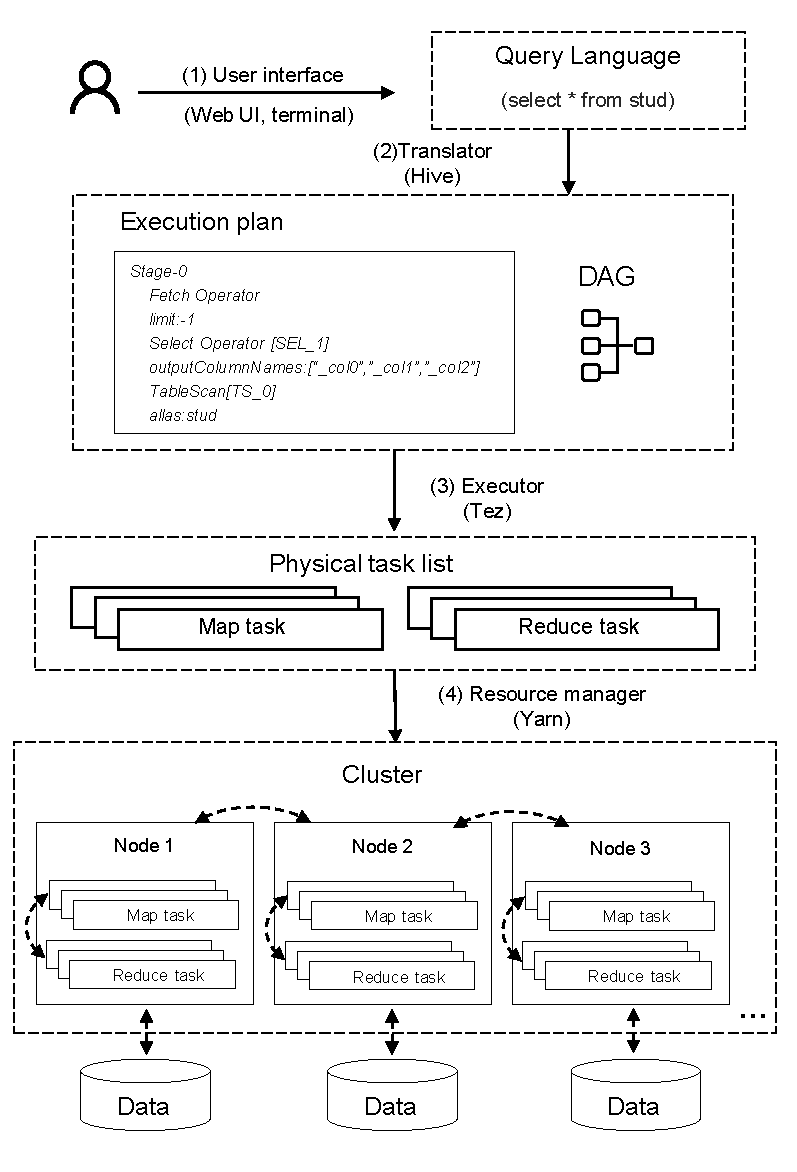
\includegraphics[width=0.42\textwidth]{figures/background/background.pdf}
	\vspace{-3mm}
	\caption{Overview of distributed query pipeline(Hadoop 2.0).}
	\label{fig:architecture}
	\vspace{-3mm}
\end{figure}

When user issues a query (shown as Figure~\ref{fig:architecture}(1)) through the interface such as a web-based user interface or SQL terminal. 
Hive uses a cost-based optimizer to optimize the query such as determining the best methods for scan operators, join orders and aggregate operation, and then translate it as the logic execution plan shown as Figure~\ref{fig:architecture}(2). The logic exaction plan may contains hundreds of lines of description, which describes the execution process as a Directed Acyclic Graph(DAG) that can be processed by the executor(e.g., Tez). 

A DAG is a collection of vertices and edges. Logically, a \textbf{vertex} consists of a sequence of logical operators(such as filter, aggregate, etc) which describes the execution of a part of the query. Further more, there are two types of vertices in the Tez DAG, \textbf{map} vertex and \textbf{reduce} vertex.  
In the DAG,  the \textbf{edges} define the data movement between the adjacent vertices. We name of source vertex as the \textbf{producer} vertex and the target vertex as the \textbf{consumer} vertex. Noticed that a producer vertex may connect to multiple consumer vertices and a consumer vertex could be connected by multiple producer vertices.  

With a given vertex, Tez further creates a set of atomic \textbf{tasks}(shown as Figure~\ref{fig:architecture}(3)). Then these tasks will be dispatched on the physical machines by Yarn, the resource manage tool of Hadoop2.0. A task takes a piece of data as input and execute all operators defined in the corresponding vertex. To ease the analysis of tasks, we define the sub-processes of a task as five steps. For a map task, the steps are \textit{Initialization}, \textit{Input}, \textit{Processor}, \textit{Sink}, \textit{Spill}. For a reduce task, the second step is \textit{Shuffle} instead. Moreover, the data read by a task could come from the local file or producer tasks.
